\documentclass[a4paper, 11pt, oneside, polutonikogreek, spanish]{article}
\usepackage[T1]{fontenc}
\usepackage{Alegreya} %% Option 'black' gives heavier bold face 
\renewcommand*\oldstylenums[1]{{\AlegreyaOsF #1}}

% Load encoding definitions (after font package)

\usepackage{textalpha}

\usepackage{listings}
\lstset{basicstyle=\ttfamily}

% Babel package:
\usepackage[spanish]{babel}

\usepackage[dvipsnames]{xcolor}
\usepackage{eso-pic,graphicx}
\usepackage[top=40mm, bottom=50mm, outer=50mm, inner=50mm]{geometry}
\setlength{\columnsep}{90pt}

\definecolor{customColor}{RGB}{213, 246, 251}

\usepackage{sectsty}
\usepackage[titles]{tocloft}

\usepackage{setspace}
\onehalfspacing

% With XeTeX$\$LuaTeX, load fontspec after babel to use Unicode
% fonts for Latin script and LGR for Greek:
\ifdefined\luatexversion \usepackage{fontspec}\fi
\ifdefined\XeTeXrevision \usepackage{fontspec}\fi

% "Lipsiakos" italic font `cbleipzig`:
\newcommand*{\lishape}{\fontencoding{LGR}\fontfamily{cmr}%
		       \fontshape{li}\selectfont}
\DeclareTextFontCommand{\textli}{\lishape}

\usepackage{booktabs}
\setlength{\emergencystretch}{15pt}
\usepackage{fancyhdr}
\usepackage{microtype}

% change color of text, example replace all \color{Goldenrod} with \color{lightgray}

\makeatletter % change only the display of \thepage, but not \thepage itself:
\patchcmd{\ps@plain}{\thepage}{\bfseries\large\color{customColor}{\thepage}}{}{}
\makeatother

\color{customColor}

\begin{document}
\bfseries
\renewcommand\thefootnote{{\bfseries\arabic{footnote}}}
\let\oldfootnote\footnote
    \renewcommand{\footnote}[1]{\oldfootnote{\bfseries#1}}
\AddToShipoutPictureBG{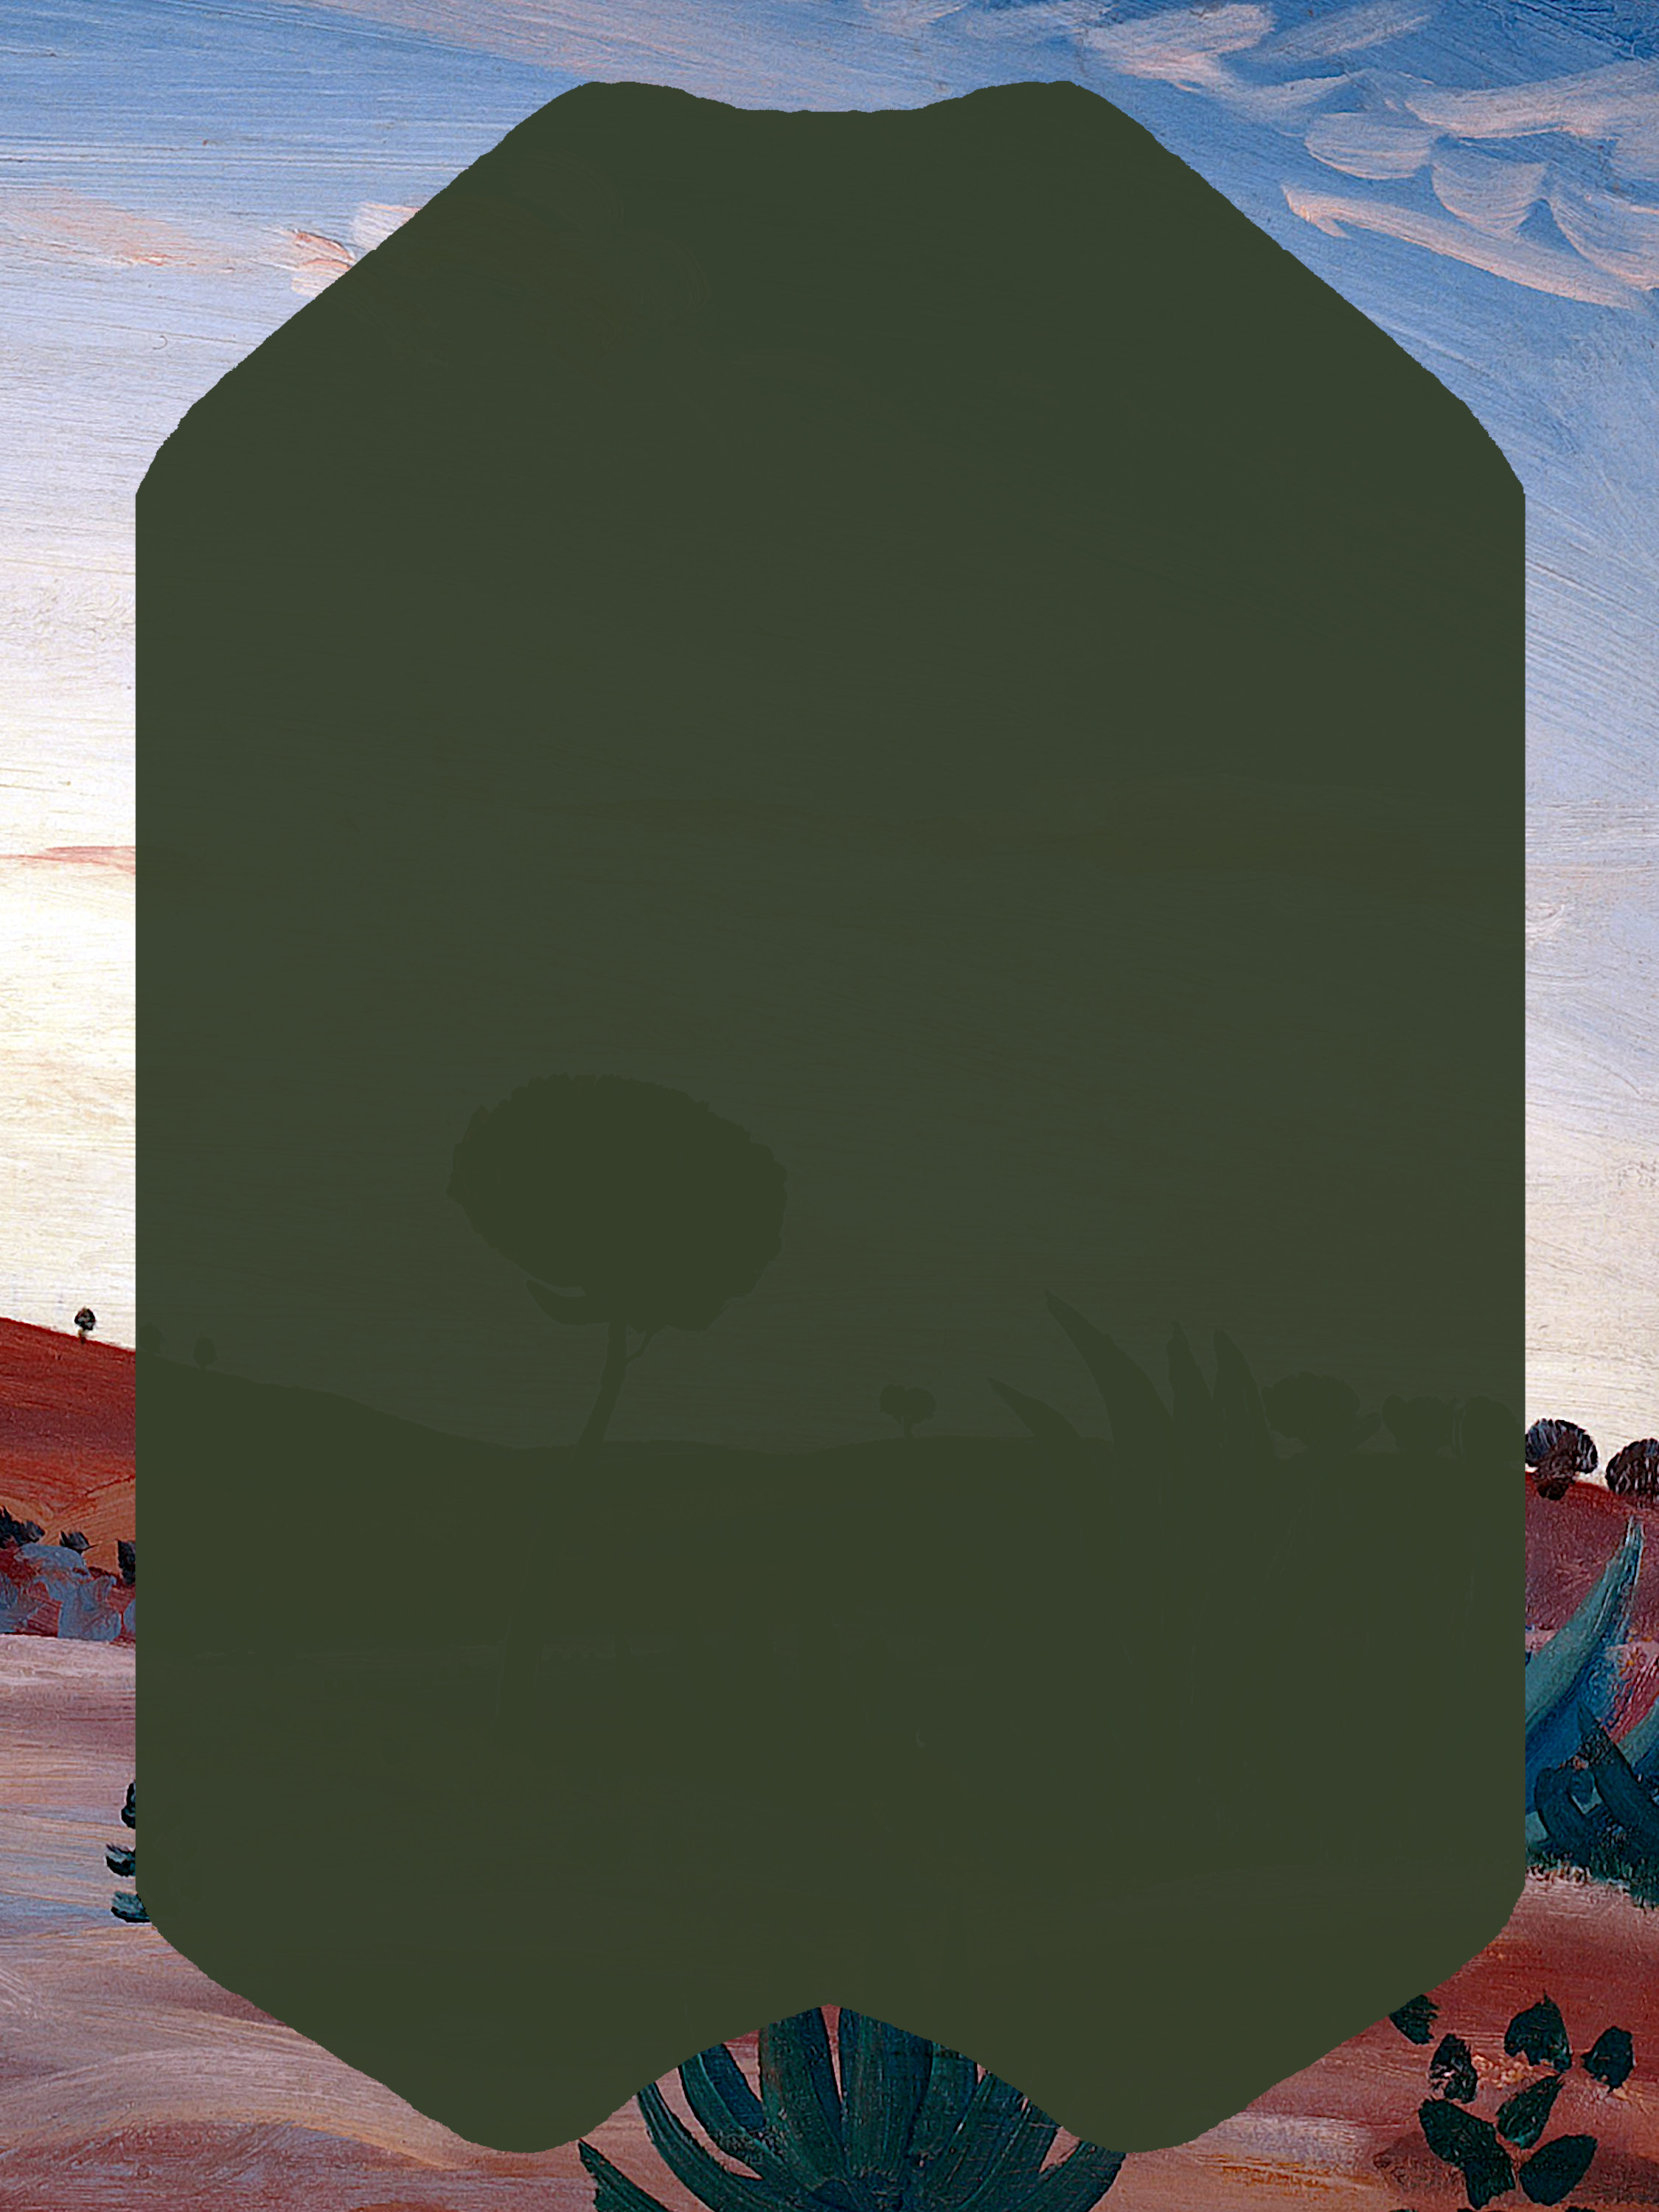
\includegraphics[width=\paperwidth,height=\paperheight]{spain2.jpeg}}
\begin{titlepage} % Suppresses headers and footers on the title page
	\centering % Centre everything on the title page
	%\scshape % Use small caps for all text on the title page

	%------------------------------------------------
	%	Title
	%------------------------------------------------
	
	\rule{\textwidth}{1.6pt}\vspace*{-\baselineskip}\vspace*{2pt} % Thick horizontal rule
	\rule{\textwidth}{0.4pt} % Thin horizontal rule
	
	\vspace{1\baselineskip} % Whitespace above the title
	
	{\scshape\LARGE Análisis de una Piedra Meteórica \\Caída en las Inmediaciones de Sixena, \\en Aragón, \\el 17 de Noviembre de 1773}
	
	\vspace{1\baselineskip} % Whitespace above the title

	\rule{\textwidth}{0.4pt}\vspace*{-\baselineskip}\vspace{3.2pt} % Thin horizontal rule
	\rule{\textwidth}{1.6pt} % Thick horizontal rule
	
	\vspace{1\baselineskip} % Whitespace after the title block
	
	%------------------------------------------------
	%	Subtitle
	%------------------------------------------------
	
	{\scshape \Large Por D. Louis Proust} % Subtitle or further description
	
	\vspace*{1\baselineskip} % Whitespace under the subtitle
	
        {\scshape\normalsize Catedrático del Real Laboratorio de Química de Esta Corte; Socio Correspondiente del Instituto Nacional de Francia; de la Real Academia Medica de Madrid, de Sevilla, Alicante, \emph{etc.}; de la Real Sociedad Cantábrica, de la de Amigos del País, \emph{etc.} } % Subtitle or further description
    
	%------------------------------------------------
	%	Editor(s)
	%------------------------------------------------
        \vspace*{\fill}

	\vspace{1\baselineskip}

	{\small\scshape{Madrid}}

	{\small\scshape Año de 1804}
		
	\vspace{0.5\baselineskip} % Whitespace after the title block

        \scshape Internet Archive Online Edition  % Publication year
	
	{\scshape\small Licencia seleccionada Reconocimiento 4.0 Internacional} % Publisher
\end{titlepage}
\setlength{\parskip}{1mm plus1mm minus1mm}
\clearpage
\large
\paragraph{}
Nadie duda ya hoy de que han caído piedras de la atmósfera en diversos puntos de la tierra. La antigüedad nos cita repetidas veces este fenómeno, y los siglos más próximos a nosotros han depositado también en sus anales la época y las circunstancias de semejantes caídas. En nuestros mismos días se han recogido en las Indias orientales, en América, en Escocia, en Inglaterra, en Francia, en Italia, en Hungría, y en fin en España, piedras o minerales, a quienes se ha dado el nombre de meteóricos. Para que nada falte al convencimiento de los que reusaban dar fe al testimonio reunido de todos los siglos y de todos los países, parece que la naturaleza ha ordenado expresamente la admirable renovación de este fenómeno, poco tiempo hace en las cercanías del \emph{Aigle}, en la Provincia de Normandía.

El año pasado de 1803 cubrió una lluvia de estas piedras una extensión de tres quartos de legua de largo sobre media de ancho. El Instituto nombró al instante un comisionado que fuese a reconocer el hecho al mismo paraje en que había sucedido, para que confirmase su autenticidad confrontando las circunstancias con la deposición de los testigos, y para que trajese á Paris una porción de las mismas piedras.

Como inmediatamente que se descubre una producción nueva en mineralogía, el primer trabajo que se emprende es el análisis químico, el Presidente de la Sociedad Real de Londres, y los particulares que conservaban algunas de las piedras en sus gabinetes, se apresuraron a remitirlas a Mr. Howard, miembro de la Sociedad, para que las analizase, y las clasificase después según las partes constituyentes que encontrase en ellas.

Pero cuál fue la admiración de este químico, cuando descubrió que las piedras caídas en puntos de la tierra tan distantes como lo están Benares en la India, la Escocia, Portugal, Italia, \emph{etc.}, se hallaban sin embargo compuestas de elementos perfectamente semejantes, aunque con alguna diferencia en sus proporciones, y que a una singularidad tan inesperada reunían también la de contener, así unas como otras, una porción notable de hierro aliado con el níquel, especie de combinación o aligación que la constitución habitual de todas las partes de la tierra que conocemos excluye de todos los minerales que encierra. La identidad de las piedras meteóricas anunciada por Howard ha sido confirmada por los trabajos posteriores de Vauquelin, con los cuales ha multiplicado las pruebas, pues que ha hallado en todos los mismos elementos, el mismo modo de combinación, y los mismos caracteres. Una semejanza tan extraordinaria entre estas piedras, y entre los fenómenos meteóricos que acompañan su caída, ha hecho concluir a todos los sabios, que unos cuerpos formados de los mismos factores, y dotados de propiedades semejantes, debían por necesidad tener un origen común. ¿Pero cuál es este origen? ¿Pertenecen a la tierra en que se precipitan... á la atmósfera de donde caen... o son arrojados por los volcanes de la luna hasta nuestra atmósfera? He aquí las cuestiones que se agitan hoy entre todos los físicos de Europa, y que el Doctor Izarn ha recogido en una obra que ha intitulado \emph{Litologia atmosférica}, impresa en Paris en 1803.

El Real Gabinete de Historia natural de Madrid posee también una de estas piedras desde el año de 1774. El Excelentísimo Señor Ministro de Estado Don Pedro Cevallos, persuadido de que ésta debía concurrir con todas las demás á ilustrar por su parte un hecho tan admirable de historia natural, me ha dado su permiso para analizarla. El resultado de mi trabajo, que presento al público, va a mostrarnos en la piedra de Sixena, que un individuo de esta prodigiosa familia ha venido a caer en España, para multiplicar con la identidad de sus elementos las pruebas de un fenómeno, cuya posibilidad han disputado largo tiempo las luces de nuestra razón.

Como el peso de esta piedra era aún bastante considerable, a pesar de los menoscabos que sufrió antes de llegar al Ministerio, para poder separar de ella algunos pedazos sin destruirla, ha ordenado S. E. que se coloque en un paraje del gabinete, bien a la vista, para que todas las personas, a quienes la lectura de las obras extranjeras y esta memoria dispertasen el deseo de verla, pudiesen satisfacer su curiosidad, y para que sirva también de punto de comparación con las que, en adelante, puedan llegarnos de la América o de España misma.

Comenzaremos nuestro trabajo por copiar la carta con que el Capitán General, que a la sazón era de Zaragoza, remitió la piedra de que tratamos, que seguramente está escrita con mucho juicio y exenta de preocupaciones. Dice pues:

«Excelentísimo Señor = Muy Señor mío. En Noviembre último se habló en esta capital de un suceso acaecido el 17 del referido mes en la Huerta de Sena, lugar del territorio de Sixena, siendo éste, que a medio día, estando la esfera celeste sin aparato de tempestad, se oyó por tres veces un ruido extraordinario, a cuyo sonido daban diversas explicaciones, y que en seguida había caído una piedra de nueve libras y una onza de peso, a la inmediación de dos hombres, que uno de ellos se acercó, y lo retrajo el olor fétido que sintió, que después, reparado del susto, la tocó con la azada de que se servía para su labor en la tierra, que él mismo fue a poner sobre ella una mano, y la retiró por estar muy caliente, y que al fin, templándose más, la recogió, y la llevó en su chupa á Sena, habiéndola presentado al Cura, el que se quedó con ella.»

«No me pareció mirar con indiferencia este fenómeno; y después de haber hecho conversación de él con varios sujetos de conocida erudición, me determiné a prevenir a la justicia de Sixena, que hiciese una información formal del suceso, y me remitiese la piedra con seguridad de ser la misma de que se trata.»

«En cumplimiento de mi disposición, me envió la información el Alcalde de Sixena, y la piedra en una caja sellada con las armas del Monasterio de Religiosas del Orden de San Juan, de cuyo Señorío es el territorio, y las mismas Religiosas me enviaron otro pedacito de piedra igual a la grande, que se cree parte de ella, por medio del Recibidor de Malta en este Reyno.»

«Luego que tuve la información y el cajoncito, abrí éste en presencia del muy Reverendo Arzobispo, de Don Juan Tomás de Micheo, Regente de esta Real Audiencia, y de los Oidores de ella Don Miguel de Villava, y Don Felipe de Rivero, que la casualidad hizo que concurriesen a un propio tiempo en el Palacio de S. M. en que resido: se vio la piedra, y se discurrió sobre su especie, caída, y otras circunstancias, resultando de esta conversación que se encargase a Don Miguel de Villava que hiciese algunas preguntas al Alcalde de Sixena.»

«El Alcalde de Sixena se dedicó a la averiguación para satisfacer a las preguntas, y me envió la información que nuevamente se le había pedido, y en ésta se halla contestado el extraordinario ruido, repetido tres veces en el día 17 de Noviembre, con admiración de unos, susto de otros, y con uniforme comprobación de él; siendo de advertir que no hay quien diga que precedió relámpago, como es regular en las tempestades.»

«Dejo á los sabios que discurran si la piedra fue erupción de la tierra, que la fermentación le dio impulso para elevarse hasta lo perceptible de la esfera celeste, y que su gravedad la precipitó al paraje en que se vio caer; si algún torbellino levantó porción de materias, que se unieron por la recíproca atracción que tendrían para juntarse, formándose la piedra, y que cayó ésta de la nube en que tuvo efecto esta operación; o que cayendo alguna exhalación mayor que las regulares, hallase la piedra en el territorio en que terminó su actividad, le comunicase su calor, la tostase en su superficie, y dejase el olor de sus materias, que se notó. Yo solo digo por mí, que el suceso, cuando no sea positivamente singular, no es común.»

«Con la segunda información me envió el Alcalde de Sixena dos pedacitos más de piedra, los cuales puse con la grande; y habiendo hecho hacer análisis, del que ya he dicho me entregó el Recibidor de Malta, se hallan las partes separadas, que contiene otro papel con rotulata que lo indica.»

«Me ha parecido, que tanto la piedra grande como las pequeñas, y la que, por medio de operaciones practicadas por perito, se halla con separación de partes, con las informaciones hechas en el asunto, merece hacerse presente al Rey; y para este fin dirijo todo a V. E. suplicándole que lo eleve a su Real conocimiento, renovando V. E. con este motivo mi veneración á los Reales pies de S. M.»

«Dios guarde á V. E. muchos años como deseo. Zaragoza 5 de Febrero de 1774. = Excelentísimo Señor, B. L. M. de V. E. su más seguro servidor = Antonio Manso = Excelentísimo Señor Don Manuel de Roda.»

Para reunir en un mismo cuadro cuanto sabemos de las piedras que han caído en España, copiaremos lo que el Bachiller Cibdareal nos dice de las que cayeron en Roa en las inmediaciones de Burgos el año de 1438.

«Al doto varón Juan de Mena, Cronista del Rey Don Juan nuestro Señor\footnote{En Roa año de 1438. Cron. cap. 275.} = Estando el Rey é todos los de la Corte cazando al pie de la cuesta de esta Villa de Roa, desque el sol se metió en unas nubes blancas, se veían bajar unos cuerpos a manera de peñas pardas, é más oscuras, é tanto espesas é grandes, que todos vieron gran maravilla. E después de colar una hora paró todo, é el sol se tornó á descubrir, é fueron unos buitreros en sus rocines á dó cayera aquella cosa, que a media legua escasa sería; é volvieron a decir, que todo el campo cubierto era de peñas grandes é chicas, que la dehesa no se veía. El Rey tobo voluntad de ir a lo ver; é le dijeron, que lugar que el cielo escogiera para sus operaciones, non era seguro andar Su Señoría fasta que otro lo viese especulado. E mandó el Rey ir a saber lo cierto al Bachiller Gomez Bravo su Adalid: é fue, é tornó estando el Rey vuelto a Roa, é trajo cuatro de aquellas peñas, é yo era presente a ello, que al verlas caer no fui presente, ca en Roa quedara. E son de los prodigios mayores que leemos en ningún Filósofo o Físico que escrito haya, que son algunas como morteros redondos, é otras como medias almohadas de lecho; é otras como medidas de medias fanegas, tanto leves é sutiles de levantar, que las más grandes media libra no pesan, é tan moles é blandas, que a las espumas del mar espesadas semejan, ca si dan a uno en la mano no le facen ferida, ni dolor, ni señal. El Rey os manda levar destas espumas o piedras. E muchos facen ya agüeros; ca no hay cosa de la natura que no la quieran semejar a la gobernación los que della son mal acomodados. = Nuestro Señor, \emph{etc.}»

Resulta de esta descripción, que dichas piedras debían ser de una naturaleza extremamente diversa de la que cayó en Sixena, y aun de cuantas conocemos hasta el día; pues que ninguna descripción de ellas nos ofrece la idea de una ligereza tan extraordinaria. Aunque su gran fragilidad no nos deja esperanza de que en el día subsistan algunos fragmentos de ellas, desearíamos que las personas aficionadas a la historia natural que viven en aquellas cercanías, se tomasen la molestia de hacer sobre ello algunas investigaciones, y me comunicasen su resultado.

Esta piedra pesaba seis libras y diez onzas cuando salió del gabinete, y la acompañaba un fragmento de tres a cuatro onzas, resto de los que habían separado de ella los curiosos. Estaba salpicada interior y exteriormente de puntos herrumbrosos, que me hicieron juzgar que la habrían tenido metida en agua, sin duda para ver si experimentaba alguna alteración. Esta herrumbre, única variación que sufrió, por poco interesante que parezca a primera vista, podrá sin embargo dejarnos entrever algunas consecuencias instructivas sobre el primitivo domicilio de estas piedras. Por lo demás, pertenecen de tal manera a la familia de las que fijan en el día la atención de los naturalistas, que no se notará diferencia entre su descripción y las que Bournon, Bacheley, Howard, \emph{etc.} nos han dado de todas las piedras que han caído en las Indias Orientales, en Portugal, Inglaterra, Francia, Ítala, \emph{etc.}

La piedra de Sixena, considerada como si estuviese entera, presenta un cuerpo aovado irregular, de siete a ocho pulgadas de longitud, sobre cuatro a cinco de ancho, y de cuatro en su mayor grueso. Puede considerarse muy bien, a poco que se repare, como una pirámide triedra bastante obtusa, de caras desiguales, con la cúspide y los cortes muy redondeados, y con la base un poco deprimida en el medio, e igualmente redondeada. Tenía, como todas las de su especie, la costra negra y vidriosa, que a primera vista parece un barniz de pez; pero la fragilidad de esta costra, el rozamiento y lo mucho que en Sixena debieron haberla manoseado, le han hecho caer la mayor parte, tanto que solo la conserva hoy en el hundimiento de la base, y un poco también en las caras de la pirámide.

Al examinar esta costra o barniz, no es difícil juzgarle efecto de un fuego que nada tiene que ver con el origen de esta piedra, y en su poco grueso se reconoce también que este mismo fuego, muy enérgico sin duda, pues que ha podido vitrificar la superficie, ha sido sin embargo momentáneo, puesto que las partes metálicas y sulfuradas que se hallan inmediatamente debajo de esta costra, no han tenido tiempo de mudar de color, ni aun de perder cosa alguna de su brillo.

La que el Abate Bacheley remitió a la Academia, fue juzgada también de esta manera por los sabios que se reunieron para examinarla. El calor, decían, habrá sido bastante grande para haber fundido la superficie; pero no ha durado el tiempo necesario para penetrar en su interior.

Parece, en efecto, que todas las piedras atmosféricas ofrecen en general la misma singularidad. Algunos físicos han anunciado que caían enteramente hechas ascuas. Sin embargo, si por esta palabra debemos entender un calor tan elevado, que las pusiese \emph{rusientes}, es difícil de concebir cómo ha podido causar en la superficie de estas piedras una alteración tan considerable, cual es la fusión, sin causar por otra parte la menor novedad en la fisonomía de los elementos que se hallan de bajo de la costra. Es constante, sin embargo, que llegaban al suelo, según se dice, abrasando, es decir, bastante calientes para quemar las manos; pero si se hubiera de juzgar de las otras por la que tengo a la vista, diríamos que este calor no ha tenido bastante intensidad para hacer la piedra luminosa, y merecer el nombre de incandescente.

Nuestra piedra tiene toda la porosidad que debe hallarse en un agregado arenisco, sin cosa alguna que la sirva de trabazón, y así el aire atraviesa con la mayor facilidad cualquier fragmento que se ponga entre los labios. El eslabón no saca de ella chispa alguna, y aun pienso que las piritas que contiene, no son susceptibles de ello, por las razones que veremos más adelante.

El fondo de su color es igual al de todas las otras, a saber, un gris azulado uniforme, que es el color de un cuerpo negro aclarado por un cuerpo blanco; y el matiz, el de un compuesto terreo teñido por el hierro oxidado \emph{ad minimum}. Por lo demás, está piedra es una masa arenisca, formada de granos ovales y redondeados, los más gruesos de los cuales no pasan del tamaño de un cañamón; y entre ellos están sembradas las partículas metálicas y sulfuradas, con toda su brillantez primitiva, y sobre todo, con el viso ligero de kupfer níquel, que Bournon ha notado en otras. Examinando los granos térreos al microscopio, se descubre también, que lejos de haber sido configurados por el movimiento de las aguas, como se podría creer a primera vista; son al contrario otros tantos glóbulos, guarnecidos de puntos relucientes o cristalinos, que no permiten de manera alguna ser confundidos con la arena. Los que son globulosos, tienen por lo general una depresión en un lado, lo cual les da alguna semejanza á la semilla del \emph{ruscus hypofillum}, y por consiguiente el aspecto de esferoides, compuestas de elementos cristalinos o de moléculas dispuestas con cierto orden, aunque en sus fracturas no se advierta cosa alguna que autorice a pensarlo.

Entre las diversas opiniones que se han aventurado sobre el origen de estos minerales, llamados prematuramente atmosféricos, las más notables son: primera, que podrían ser obra del meteoro mismo, el cual, hallándose recargado de los gases de la sílice, de la magnesia, del hierro, del níquel, \emph{etc.}, habrá podido engendrarlas, como otros engendran la lluvia, combinando sus elementos por medio de su propio calor, y de las atracciones que este puede excitar. Segunda, que podrían haber sido lanzadas hasta nuestra atmósfera por la explosión de algún volcán de la luna. Pero, sin deternos a repetir las razones que se han dado para demostrar la inverosimilitud de uno y otro origen; basta comparar la textura interior de estas piedras con su costra, para abandonar toda idea de que el fuego haya podido ser jamás el agente de su formación. Si nos atenemos, en efecto, a las inducciones que pueden sacarse de la cristalización del hierro del sulfurito, de la de los glóbulos térreos que le sirven de ganga, de la brillantez, de la integridad, y en una palabra, del aspecto fresco que conservan todas sus partes, si consideramos además, que los elementos térreos y metálicos que forman esta clase de minerales, no tienen, ni en su naturaleza, ni en el modo de combinación que el análisis descubre en ellos, nada que los distinga esencialmente de todos los demás compuestos del globo, nos persuadiremos de que, lejos de ser el resultado de una operación ígnea y violenta, que lo allana y confunde todo, no han podido nacer, por el contrario, sino en medios tranquilos, y con circunstancias tan pacíficas y tan lentas, sin duda, como todos los demás minerales que componen el globo. Quitémosle, en efecto, esta costra vidriosa, este accidente que las desfigura, y que las priva de su verdadero aspecto, presentémoslas a los litologistas más diestros, y nos convenceremos muy pronto de que, entre todas las hipótesis que se pueden aventurar sobre su origen, la del fuego o de los volcanes no puede merecer siquiera contarse la última.

Salverte dice, con razón, que si estas piedras hubiesen sido lanzadas por volcanes, los metales que contienen estarían precisamente oxidados. Con la misma exactitud ha pensado cuando ha dicho, que solo una descarga eléctrica era capaz de vitrificarlas de la manera que lo están. En efecto, es preciso convenir en que el fuego, que ha podido desnaturalizar su superficie, lejos de obrar progresivamente, y como el de nuestros hornos, ha debido desplegar, por el contrario, una actividad inmensa en el más corto espacio de tiempo. Ahora, este fuego, que ha debido reunir la energía del rayo a la rapidez del relámpago, no puede ser otro que el que funde, el que oxida el oro y la platina, sin dejar en las vasijas que los contienen el menor rastro de su paso, y el mismo en fin, que puede fundir la hoja de una espada sin lastimar la vaina. En una palabra, la mejor comparación que podemos hacer de la piedra de Sixena, es con un pedazo de cera metido en un horno caldeado, y sacado inmediatamente. Su superficie se derrite, y una línea más adentro no experimenta la más leve alteración de temperatura.

Sin embargo, Salverte excede los límites de la verisimilitud cuando añade, que un golpe violento de electricidad, o un calor sumo pueden determinar la formación de las que están más vitrificadas. Si el meteoro que transporta una de estas piedras, cuyo interior no está en manera alguna fundido, aunque de una naturaleza muy fusible, es un meteoro ígneo desde su origen, no puede ser obra suya; si, al contrario, es frio hasta el momento en que se abrasa y hace la explosión que determina, al parecer, el momento de su caída, no podemos presumir con el menor fundamento que haya podido más bien formarse en esta segunda época, que el que haya sido capaz de engendrar un agregado terreo, metálico y sulfuroso; que si bien se considera, no ofrece en su composición ningún elemento nuevo para nosotros, ninguna substancia que no hallemos en los otros minerales de nuestro globo; No: tan poco exacto es el decidir que uno de estos minerales no pertenece a nuestro globo, porque los mineralogistas no le han encontrado aun sobre la superficie de la tierra registrada hasta el día, como el creer que los millones de altramuces que un huracán, según dicen, sembró en las cercanías de Leon\footnote{El año pasado publicaron nuestros periódicos esta Lluvia de Altramuces: el difunto D. Antonio Josef Cavanilles, Director del Real jardín botánico, sembró en él algunas de las muchas semillas que se remitieron a Madrid, las cuales han florecido esta primavera, y han manifestado que pertenecían al \emph{lupinus pilosus}, planta descrita por Linneo sin saber dónde se criaba, y que Don Luis Nee ha hallado en la Real Casa del Campo.} han sido creados en las regiones de la atmósfera, porque no se ha hallado en la Provincia la especie que produce dichas semillas: pero ya añadiremos á estas otras conjeturas, después de haber analizado la piedra de Sixena.
\begin{center}
\emph{Análisis.}
\end{center}
\paragraph{}
Habiendo expuesto a un calor rojo, por espacio de medio cuarto de hora, y en un crisol cerrado, un fragmento de esta piedra de cosa de dos pulgadas, salió de él extremamente alterada. Los glóbulos areniscos se habían vuelto de un color pardo mucho más obscuro, y los granos metálicos, despojados de toda su brillantez, se habían oxidado visiblemente: con el color y al grado del hierro que ha servido para la descomposición del agua. Esto nos mueve ya a asegurar, que si el interior de la piedra hubiera experimentado de parte del meteoro una incandescencia, aunque hubiese sido tan solamente de la misma duración, hubiera perdido incontestablemente la frescura y brillantez que caracteriza las partes metálicas, porque el aire que se insinúa en ella o la penetra tan fácilmente, no hubiera podido menos de ocasionar las mismas alteraciones. Pero en la piedra de Sixena sucede todo lo contrario: tiene una costra vidriosa, que no se diferencia de la que hubieran podido causarle nuestros hornos; y sin embargo, sus moléculas interiores conservan toda su integridad, todo el aislamiento que es propio de agregados que no se han acercado al fuego jamás. Este resultado confirma el juicio que hemos hecho ya de la naturaleza del fuego que han experimentado estas piedras, y nos da en alguna manera la medida del que ha sufrido, después de habernos indicado la especie.

Deseando conocer los efectos de un fuego más activo, puse a caldear en la fragua cosa de dos onzas de la piedra, por espacio de media hora, que es á corta diferencia el tiempo que hubiera tardado en fundirse un pedazo de cobre. Saqué del fuego el crisol, y hallé los fragmentos perfectamente fundidos, en una masa semividriosa, negruzca, ligeramente porosa, y que no anunciaba, según el estado de los bordes del crisol, haber experimentado mucha efervescencia antes de fundirse. Estaba sembrada de glóbulos que no habían tenido tiempo de deshacerse, aunque se había ya reunido en el fondo un regulo de más de cien granos.

Este régulo no era muy frágil; se desmenuzaba al golpe del martillo, y sus partículas, difíciles de separar, ofrecían unos hacecillos, que juzgué cristalizados, por la desigualdad de sus filamentos. El ácido sulfúrico disolvió fácilmente este hierro, y el hidrógeno que se desprendió de él, llevaba aquel olor bituminoso que caracteriza las fundiciones carbonosas. Pero nada tenía de sulfuroso, porque el azufre de las piritas, empleado, sin duda, en desoxidar una parte del hierro que tiene la piedra, debió disiparse en ácido sulfuroso: fenómeno igual al del bermellón vuelto al estado metálico por el azufre, según la teoría de Morveau. La masa vidriosa, en fin, bien nivelada en el crisol, no le había atacado sensiblemente, lo cual anuncia que la sílice, la magnesia y el oxide se hallaban en las proporciones suficientes para saturarse unos a otros.
\begin{center}
\emph{Del hierro contenido en la piedra.}
\end{center}
\paragraph{}
Las partículas que el imán separa tienen muy poco volumen para poder distinguir su figura con la lente; sin embargo, parecen octaédricas. Tampoco están distribuidas con igualdad, pues que unas veces he separado 17, otras 19, y otras en fin 22 por 100. Para lograrlas bien puras y libertarlas de herrumbre las he separado de las partes areniscas, valiéndome de espíritu de vino en vez de agua; y a pesar de esto, siempre retienen alguna porción, porque al machacar la piedra en el mortero se aplastan y arrollan algún tanto dichas partículas. Cien granos de este hierro, disueltos en ácido muriático, dejaron cinco de arena, lo cual supone cosa de siete de piedra, porque el ácido había disuelto el oxide y la magnesia.

Los granos metálicos, tratados al soplete, no exhalan olor alguno: se disuelven a la manera del hierro ordinario. El hidrógeno no les quita nada sulfuroso, puesto que no hace la menor impresión sobre el papel escrito con la disolución de plata; en fin, su disolución en al ácido nítrico no enturbia la barita. Todo esto demuestra, que el hierro que el imán separa de la piedra de Sixena nada tiene de sulfurado.
\begin{center}
\emph{Del Níquel.}
\end{center}
\paragraph{}
Siempre he encontrado este metal aliado a los granos de que acabo de hablar, y jamás en la parte lapídea o sulfurada.

La disolución muriática de cien granos, tratada con un poco de ácido nítrico, elevó el hierro al \emph{maximum} de su oxidación; pero no el níquel. Este último, aunque susceptible también de una oxidación máxima, tiene, como el de manganesa y el de cobalto, mucha afinidad con los ácidos, para que el nítrico pueda elevarle de su \emph{minimum} mientras se halla unido a un ácido. Después precipité la disolución con el amoniaco, para lograr separadamente el oxidé de hierro. En seguida le mezclé con un poco de potasa, le evaporé, y me dio secciones de prisma romboidal, de un verde hermoso y de 24 gramos de peso; y como 100 partes de sulfaté de níquel tratados con potasa contienen doce partes de metal, resulta que los 24 granos contienen cerca de tres. Haré, puesto que se presenta la ocasión, una digresión corta para exponer algunos hechos sobre el níquel, que merecen ser conocidos.

Cien partes de este metal, perfectamente purificado por los medios de que hablaré en otro lugar, disueltos en el ácido nítrico, y destilados hasta la completa descomposición del nítrate, me han dejado, por dos veces, de 133 a 134 de un oxide parecido a la escamonea en polvo.

Cien partes de dicho metal, disueltas en el ácido nítrico y precipitadas con carbonate de potasa, me han dado, por dos veces, de 232 a 233 de carbonate de níquel, de un verde pálido. Este carbonate, destilado, se reduce a 135 de oxide pardo: en esto vemos que la potasa y las lavaduras le recargan de un poco de tierra.

El ácido muriático disuelve este metal, como disolvería el hierro, y el hidrógeno que se desprende, tiene el carácter bituminoso, lo cual me hace sospechar que puede también disolver carbón. Esta disolución da también de 232 a 234 por 100 de carbonate, lo cual demuestra que el ácido muriático no oxida el níquel, así como tampoco le oxidó el nítrico.

La potasa pura precipita el oxide de níquel en un hidrate de color más obscuro que el carbonate, y que no se descompone por la ebullición, ni en el agua, ni en la potasa. Las afinidades de este oxiden con el agua son mucho más fuertes que las del oxide de cobre, y corresponden a sus otras afinidades con los ácidos. El hidrate de níquel se disuelve con calor y sin efervescencia en los ácidos; y sus disoluciones no alteran, ni las de plata, ni las de barita. Deja destilándole 78 por 100 de oxide pardo, porque contiene 22 por 100 de agua, sin gas alguno. Tiene también el carácter de exigir que se le caliente por más tiempo y con más fuerza que el de cobre, para privarle completamente de agua. El hidrate destilado no cede cosa alguna al agua; sino, a veces, algunos átomos de sulfate de potasa, que no hacen impresión en la tintura del tornasol pero que son sensibles a la barita.

El oxide de níquel tiene, como el de cobre, y verosímilmente como otros muchos, la propiedad de dar con el ácido sulfúrico combinaciones, que puedan hallarse con agua o sin ella.

Cien partes de sulfate de níquel destiladas pierden 24 de agua, y se reducen a un polvo de color amarillo de canario, que puede entrar en una fusión roja, sin variar de estado ni de color. Este polvo amarillo extendido sobre e el papel atraje la humedad, y vuelve a adquirir el hermoso color verde del sulfaté.

El sulfate de cobre destilado da un polvo de un color blanco puro; pero exponiéndole a la humedad de la atmósfera o del aliento, vuelve a tomar su color azul, y se convierte otra vez, como el del níquel, en un sulfate cristalizable y coloreado. Los sulfates pueden pues tener o no agua, y la expresión de Chenevix, que ha dicho que el sulfate de cobre era la disolución del hidrate en un ácido, es de todo punto exacta.

Se ha observado, que la denominación de hidrate no podía convenir a un compuesto que tenía por uno de sus factores el hidrógeno oxigenado, porque no es ácido; pero la acidez es también un atributo muy variable en el producto de los otros combustibles quemados. ¿Qué sabor tiene, por ejemplo, el ácido boracico bien puro? (y para serlo es preciso haberle fundido) una acidez que la lengua no puede descubrir, y que solo la indica el tornasol. Sin embargo, sus combinaciones son para nosotros borates. El oxide de tunstena no es seguramente ácido; y sin embargo, se admiten sin escrúpulo sus tunstates, porque son unas combinaciones muy regulares y muy cristalizables. No puede negarse que el agua se combina hasta saturación, y se condensa uniéndose con la cal: y a no ser por el color blanco de esta combinación, que nos impide el notar, como en los oxides coloreados, los caracteres nuevos que el agua le imprime, hace ya tiempo que yo hubiera colocado la cal apagada en la línea de los hidrates, lo mismo que la potasa que perdió la propiedad de calentarse con el agua, y que cristaliza regularmente, si está combinada con cierta cantidad de ella; porque si existen combinaciones del agua con los oxides, no podemos menos de admitir la posibilidad de una combinación igual entre el agua y las bases que tienen más atracción con ella que los oxides. Y en fin, si los oxides pueden todos dar combinaciones salinas, con agua o sin ella; los álcalis vemos que nos ofrecen combinaciones de este mismo género en muchas sales neutras. Pero volvamos al níquel.

Su oxide pardo, su carbonate y su hidrate descomponen el ácido marino oxigenado, y se convierten en un polvo de un color violado obscuro, que parece negro cuando está seco. Este oxide, que acaso se hallará en la naturaleza, se porta del modo siguiente con los tres ácidos: en el muriático da en abundancia el gas muriático oxigenado, y en el sulfúrico y el nítrico se disuelve con efervescencia, y da gas oxígeno. Las disoluciones que provienen de él son verdes, y contienen el oxide \emph{ad minimum}, que es el estado ordinario de las disoluciones de este metal. No conozco numéricamente el grado de oxidación del níquel. Este metal, que en efecto es muy atraído por el imán, tiene con el hierro una semejanza de que haré mérito; porque puede ser útil en el análisis de sus minas. Su oxide, calentado hasta enrojecerle, con un poco de aceite, en un crisol cerrado, se reduce muy fácilmente, se vuelve atraíble, toma el color metálico, y su fusión exige un fuego que no me parece superior al que derrite el hierro colado.

El cobalto sigue en todos sus puntos la marcha del níquel. Los ácidos le oxidan uniformemente. Da hidrate, da oxide pardo, cuando está oxidado \emph{ad minimum}, y negro cuando ha sido sobre-oxigenado por el ácido muriático oxigenado. Este nuevo oxide se disuelve con las mismas circunstancias que el del níquel. Yo pienso que los oxides nativos de cobalto, que son muy negros, podrían muy bien presentárnosle sobre-oxigenado. El cobalto en fin, muy atraíble, se funde con suma dificultad: ya diré en otra parte cómo he logrado purificarle. Sigamos con la piedra de Sixena. Aunque el amoniaco merezca la preferencia sobre la potasa para separar el hierro del níquel, esta puede sin embargo, servir para ello con la misma ventaja, porque la fuerza con que los ácidos atraen el oxide rojo, es muy inferior a aquella con que atraen los oxides de níquel, de cobalto y de manganesa. Hay pues siempre, entre el punto en que el hierro acaba de precipitarse, y el en que estos últimos comienzan a hacerlo, un intervalo bastante notable, para poderlos separar sin riesgo de confundirlos. Este modo de aplicar la potasa es sobre todo extremamente útil en la purificación en grande del níquel y del cobalto.

Todo esto nos enseña, pues, que el hierro separado por el imán de la piedra de Sixena es, como todos los de las otras piedras de este género, una aligación en que entra el níquel; aligación muy propia para confirmar la analogía que Howard ha notado entre el hierro de las piedras meteóricas y las asombrosas masas de hierro que se han encontrado en Siberia y en el Tucuman; y en las cuales este químico ha hallado, como yo, el níquel. Considerando, en efecto, su composición y su situación sobre la tierra, no podemos dudar ya hoy, que los meteoros que acaban de arrojar estas piedras a miles en Normandía, y que en una multitud de parajes las han dejado caer de 100, de 260 y de 300 libras de peso, hayan podido con la misma facilidad arrojar masas de 14 quintales de esta aligación.
\begin{center}
\emph{Acción del agua sobre la piedra.}
\end{center}
\paragraph{}
Puse en agua destilada un fragmento de cosa de dos pulgadas, por espacio de doce horas, y al día siguiente le saqué cubierto de manchas herrumbrosas, que sirvieron para indicar el sitio de los granos de la aligación, que antes no se podían distinguir de los que estaban sulfurados. Estos últimos habían conservado su brillantez.

El agua ácida el fondo de la vasija estaba teñido de un color ligero de café, que me sorprendió por el pronto. No era una disolución de hierro, porque el prusiato de potasa no varió en nada su matiz; pero inmediatamente que le añadí algunas gotas de ácido marino, desapareció el color. El oxide, que estaba allí solo diluido en el agua, tomó inmediatamente el estado salino, y se convirtió en azul de prusia añadiéndole prusiato de potasa; pero no es esto solo; el oxalato de potasa, y el muriato de barita descubrieron en esta agua señales bien notables de ácido sulfúrico y de cal. Vauquelin y Klaproth han notado también la existencia de esta tierra; pero en cuanto al ácido sulfúrico que no existía en la piedra, se juzga bien que la combustión de los granos sulfurados que estaban en su superficie, debió rodearla de una atmósfera que tuvo tiempo de penetrar en sus poros.

En cuanto a la facilidad con que se pone herrumbrosa, veremos más adelante las consecuencias a que puede conducirnos esta alteración.

%trailing section header
\clearpage
\begin{center}
\emph{Acción de los ácidos.}
\end{center}
\paragraph{}
El ácido sulfúrico, y el nítrico muy debilitados, dividen y analizan tan fácilmente la parte terrea de nuestra piedra, como los que están más concentrados. El ácido muriático la disuelve también, y separa de ella de 66 a 67 centésimos de sílice. Con el auxilio de este ácido se desprende también un hidrógeno sulfurado sin mezcla de ácido carbónico, y que apenas contiene una cantidad sensible de hidrógeno puro. Hablo aquí de la piedra de la que se han separado por medio del imán las partes atraídas por él. Esta disolución forma a veces una jalea, a causa de la sílice.
\begin{center}
\emph{Del sulfurito de hierro contenido en la piedra.}
\end{center}
\paragraph{}
Cien partes de nuestra piedra purgada de hierro, tratadas en una retorta con agua regia, y reunidas al producto de la destilación, han dado con el muriato de barita 16 granos de sulfate, que según la estimación de Chenevix pertenecen a 46 de azufre. La combinación que este azufre produce aquí con una parte del hierro de la piedra, no es como muchos químicos lo han pensado, una pirita común, puesto que este sulfurito natural no cede a la acción de los ácidos sulfúrico y muriático hasta el punto de formar hidrógeno sulfurado; diferencia que no se le pasó a Howard; y los químicos que analizaron la piedra del Abate Bacheley observaron también que el olor hepático acompañaba a su disolución.

En el hierro existe el azufre en dos proporciones, que me parecen constantes, tanto en el arte como en la naturaleza. La 1a. es de 60, y la 2a. de 90 sobre 100. La 1a. se obtiene combinando directamente el hierro con el azufre, según el método que seguimos para preparar el sulfurito que nos provee de hidrógeno sulfurado. Se obtiene también destilando las piritas, lo cual rebaja el azufre que contienen de 90 a 60 sobre 100 como lo haré ver en otra ocasión. La 2a. proporción es siempre obra de la naturaleza, aunque he logrado imitarla, como puede verse en la memoria que he dado sobre la pirita. Pero la 1a., si existe en nuestras minas, no se ha presentado todavía a nosotros; y si la encontramos hoy en las piedras meteóricas, podemos, a mi entender, decir que es la primera vez que la naturaleza pone a nuestra vista el sulfurito de hierro \emph{ad minimum}. Volviendo pues al azufre de nuestra piedra, podemos concluir de lo que hemos dicho, que la cantidad de 4, 6 que hemos descubierto, establece en ella una cantidad de 12 de sulfurito \emph{ad minimum}, porque las combinaciones del arte siguen, en general, tan de cerca las de la naturaleza en sus proporciones, que creo podamos, admitir esta relación mientras se nos presenta una verificación más exacta.

El amoniaco aplicado a la disolución nítrica de nuestra piedra ha precipitado de ella 18 centésimos de oxide rojo de hierro; pero si separamos 12 por las 8 partes de hierro que servían de base al sulfurito, nos restarán 6 para el que pintaba la piedra; y como su color es el que da el oxide \emph{ad minimum}, y no el oxide rojo, se puede suponer también que el oxide negro no excede en ella de 5 centésimos. En todo análisis me parece preferible el calcular el hierro por la cantidad de su oxide rojo, porque este último es invariable, y puede soportar un calor rojo sin perder oxígeno.
%trailing section header
\clearpage
\begin{center}
\emph{Manganesa.}
\end{center}
\paragraph{}
El líquido, privado de hierro y sin exceso de amoniaco, punto esencial de observar para lograr con seguridad el oxide siguiente, le trate con el hidro-sulfurito de amoniaco. Quemé en una cuchara de platina el precipitado que obtuve, y fundiéndole después con un poco de bórax le tiñó, con mucha admiración mía, de un color legítimo de manganesa. Para asegurarme más de un metal, que según yo esperaba, debía ser el níquel, emplee de nuevo 800 granos de piedra purgada de hierro por el imán, y separé después el oxide rojo por medio de la potasa. Acabé la precipitación con el prusiato, y el precipitado, en vez de ser verde, como el del níquel, se presentó con un matiz de flor de melocotón, que es efectivamente el de la manganesa. Este prusiato quemado tiñó abundantemente el bórax del color violado que yo debía esperar. Pero como el oxide de manganesa está en nuestras piedras en una cantidad muy pequeña, no he tratado de deducirle de su prusiato, porque esto exigía verificaciones á que no he tenido tiempo de dedicarme. Solo sé, por una serie de experimentos repetidos, que el prusiato de potasa cristalizado tiene en todos los prusiatos metálicos, y por consiguiente en el azul de prusia, de 30 a 31 por 100 de prusiato blanco, es lo mismo, el oxide que es su base: y que es también en el azul de prusia un elemento tan esencial a su existencia, como a la del prusiato de potasa cristalizable.

En cuanto al prusiato de hierro, compuesto de oxide rojo y de ácido prúsico exclusivamente es una combinación nueva, esencialmente diversa del azul de prusia. Esto causará, como se puede juzgar, una gran modificación á la memoria que he dado sobre los prusiatos; pero mientras puedo repetir este trabajo, diré, para los que deseen entrar en la nueva ruta que deben abrir los prusiatos metálicos puros, que el de hierro es verde; que se obtiene con el sulfate rojo y el prusiato de potasa puro descrito por Schele, quien con una multitud de hechos indispensables para su conocimiento nos ha puesto hace mucho tiempo en camino de conocerle bien: más casi no ha quedado vestigio de ellos entre nosotros; que este prusiato soluble en el ácido sulfúrico o en un exceso de sulfate rojo, que como se sabe es siempre ácido, le comunica el color rojo de sangre, que notamos constantemente en las lexías que han servido o que quedan de la formación del azul de prusia; que se obtiene una buena cantidad de prusiato de potasa puro, aplicando el espíritu de vino a las lexías concentradas de carbón animal fundido con la potasa, lo cual le separa del carbonate, del sulfate y del prusiato de potasa cristalizable, que estas lexías deben al hierro de la sangre, y que ellas jamás contienen sino en una cortísima cantidad; y en fin, que al contrario de lo que he establecido en mi memoria. Sino se usase, como se hace del sulfate ordinario del comercio, que es siempre una mezcla de los sulfates rojo y verde, y tiene por consiguiente la ventaja de ceder al prusiato de potasa puro la porción de oxide verde que necesita para pasar al estado de prusiato cristalizable, no se obtendría una cantidad considerable de azul de prusia, porque este último no se forma sino en cuanto el prusiato cristalizable puede trasmitirle oxide verde, que para él es un elemento indispensable, elemento que por consiguiente se encuentra entero en el azul de prusia, elemento que el oxígeno nítrico o atmosférico no podrían sobre-oxidar en él, elemento en una palabra, que el prusiato de potasa, es incapaz de trasmitirle, pues que él mismo no le tiene.
%trailing section header
\clearpage
\begin{center}
\emph{Cal.}
\end{center}
\paragraph{}
La cal se encuentra también en nuestras piedras, como hemos dicho al principio, pero en una cantidad tan corta, que es difícil graduarla, a menos que se opere sobre 600 u 800 granos de materia. La disolución sulfúrica, por ejemplo, privada del exceso de ácido y concentrada, da entonces unos filamentos de sulfate de cal, primero que el de magnesia. En cuanto a la arcilla, no creo que la haya, al menos no he descubierto rastro de ella, ni aun buscándola directamente.

Si resumimos estos resultados, descubrimos en primer lugar, que el níquel no está ni sulfurado ni oxidado en la piedra de Sixena. Está aligado solo al hierro, y esta es la aligación que el imán separa de la piedra reducida a polvo. En cuanto al oxide negro de hierro, que es a quien debe la piedra su color gris, también le acompaña el de manganesa, como sucede en tantos otros compuestos lapídeos. Aun presumo que los que en adelante analicen piedras meteóricas, le hallarán también en ellas, sobre todo si no las tratan \emph{colectivamente}, lo cual perjudica a la sencillez del trabajo. La magnesia la he encontrado siempre en la proporción de 19 a 20 centésimos. Podemos según esto formar la tabla siguiente, que solo será de aproximación, atendiendo a la dificultad de las valuaciones rigurosas en los análisis.
\begin{table}[!h]
    \centering
    \bfseries
    \begin{tabular}{l r}
        Sulfurito de hierro \emph{ad minimum} & 0,12 \\
        Oxide de hierro negro & 0,05 \\
        Silice & 0,66 \\
        Magnesia & 0,20 \\
        Cal y manganesa. átomos. & 0,00 \\ \hline
         ~ & 103 \\
    \end{tabular}
\end{table}
\paragraph{}
No he creído deber colocar en este resultado el hierro que el imán puede separar de él, porque solo está interpuesto en la piedra, al modo que lo están los metales vírgenes en su \emph{ganga}: y así lo analizamos siempre aparte cuando la separación mecánica nos facilita los medios de hacerlo. Además de eso este modo de ver ofrece ciertas semejanzas que pueden tener su utilidad. Establecen entre los minerales meteóricos y los del globo conocido una analogía de estructura y de composición, que no hubieran dejado de advertir los naturalistas que los han estudiado, si el deseo de buscar su origen en las regiones de las maravillas, más bien que en las de lo verosímil, no les hubiera extraviado del camino que podía conducirlos a esto.
\begin{center}
\emph{Consecuencias.}
\end{center}
\paragraph{}
En el discurso de este análisis se ha podido ver, que comparando las piedras meteóricas con los minerales del globo conocido, he procurado llamar la atención sobre las analogías que aproximan las primeras a las segundas. ¿Sería en efecto imposible o inverosímil que las piedras que no se presentan en las regiones conocidas, y que ni aun podrían encontrarse en ellas por las razones que veremos al instante, perteneciesen sin embargo a las que el hombre no conoce todavía, y 4 que probablemente no se acercará jamás? ¿No parece, por ejemplo, que antes de ir a buscar a la atmósfera o a los volcanes de la luna un origen, á compuestos que no tienen un elemento siquiera que los excluya de los del globo, nos debíamos detener primero en la posibilidad que hay de que pertenezcan a la inmensa porción de tierra que rodea los polos? ¿y por qué unos meteoros cuyo, origen no conocemos, ni los combustibles que contienen, ni el impulso que los mueve, ni la naturaleza de las líneas que recorren, han de ser menos a propósito para arrancarlos de cualquier punto del globo que para formarlos, contra toda verosimilitud física, de unos elementos que ni la atmósfera puede crear, ni conservar en disolución?

Procuremos reunir algunas de las luces que el análisis puede ofrecernos.

La costra que estas piedras tienen es un accidente. En esto no cabe duda; una causa extraña ha desfigurado visiblemente su superficie, como hubiera podido hacerlo el calor de un horno de cal con un trozo de piedra arenisca o de granito que cayese en él, y que cubriera de un baño vidrioso; y esta causa es necesario reconocer también, que no ha podido explicar sobre la piedra más que una actividad muy momentánea, porque si hubiera tenido tiempo de propagar sus efectos más adentro, no hubiera dejado de reducir a vidrio un agregado de una naturaleza tan fusible como estas piedras.

Esta causa no puede ser por otro lado sino el fuego mismo del meteoro que las trasporta, y que unas veces se anuncia enteramente encendido desde el principio del horizonte en que se comienza a percibir, otras también no parece que se inflama hasta después de haber surcado una porción de la atmósfera bajo el aspecto de un cuerpo obscuro, cuya causa se termina con la explosión que precede a la caída de las piedras. Pero en cualquier época que se consideren estos globos que una acumulación del fluido eléctrico obliga a precipitarse, se conoce con la misma evidencia, que no han podido engendrar estos minerales por la sola fuerza de la ignición, porque la naturaleza y la combinación de sus elementos la disposición de estas mismas combinaciones, y la organización interior de estas piedras no tienen cosa alguna que no repugne, bajo todos aspectos, a las ideas que tenemos de esta misma ignición, nada en una palabra que pueda asemejarlas a producciones volcánicas.

Es preciso según esto concederles dos épocas bien distintas: la primera será aquella en que los minerales yacían pacíficamente, no diré ni en qué paraje, ni en qué espacio; pero siempre en un sistema de cuerpos muy distantes de tener por temperatura habitual un calor capaz de degradar su estructura; y la segunda en que después de haber sido arrancados por una causa violenta a su inercia primitiva, recorren las llanuras de la atmósfera, envueltas en el torbellino de un meteoro desconocido, que divide con ellas su movimiento para sostenerlas contra su propio peso, y que no las abandona jamás hasta haberles impreso esta degradación, que lleva el sello claro de una explosión eléctrica.

Si traemos ahora a la memoria la alteración rápida que estas piedras experimentan en la humedad, no podremos menos de asentir a la verdad siguiente. El sistema de que hacían parte debe gozar habitualmente de una sequedad perfecta, pues que la aligación brillante y cristalizada de sus metales no podría sufrir sin oxidarse la mansión más corta en cualquier otro sistema que, como el del globo que habitamos, estuviese penetrado de una humedad que en su superficie alternase con la sequedad, pero que si puede decirse así, sea un estado habitual para todos los minerales colocados debajo de esta superficie. Se concibe, en efecto, que una piedra meteórica abandonada en nuestros climas a las variaciones que sufre la superficie de la tierra, no podría dejar de padecer tanta degradación en sus partes metálicas como un pedazo de hierro bruñido, y que esta degradación debe hacer hoy desconocidas un gran número de estas piedras, que habrán permanecido sobre la tierra desde su caída, y que es ya imposible distinguirlas de las piedras ferruginosas que abundan por toda la superficie del globo.

Port anto, si es permitido conjeturar sin perder de vista los principios, no repugna a la razón presumir, que lejos de haber tenido su origen en medios ardientes y acuosos, puesto que la naturaleza de estas piedras excluye hasta la verosimilitud de ellos, podrán haber sido arrancadas de algunos de los puntos del globo, que no teniendo por sí, ni la humedad que refresca continuamente la superficie y el interior del suelo que habitamos, ni el calor que vivifica los cuerpos organizados manteniendo la fluidez líquida y gaseosa de las aguas, podría por consiguiente mantenerlas en este estado habitual de sequedad absoluta, que su organización interior exige invenciblemente.

Pues un sistema a propósito para conservar perennemente al hierro en aquella integridad, que puede por sí sola asegurarle el magnetismo, y defenderle de la oxidación, que es hoy el estado general del hierro en todos los climas de la tierra en que el agua goza de la fluidez, no puede conciliarse sino con las ideas que debemos tener de las tierras polares, regiones en que un frio eterno no permite jamás al agua abandonar el carácter de roca primitiva que debe tener en ellas, ni al hierro el de cuerpo combustible.

Pero en fin, conjetura por conjetura, concluyamos de las luces que el análisis nos suministra sobre la naturaleza de los minerales meteóricos, que los parajes, o el sistema de donde han sido desprendidos no puede tener por temperatura habitual, ni el calor que ha fundido su superficie, ni las alternativas de sequedad y humedad que reinan sobre las regiones templadas del globo, y que muy lejos de haber podido producirse pocos instantes antes de su caída, es infinitamente más conforme a los principios de la filosofía natural pensar que preexistían á la causa violenta que los arranca a su inercia, y que son verosímilmente tan antiguos como los demás minerales del globo.
\clearpage
\end{document}
